\section{Message from the Program Committee Co-Chairs}
\setheaders%
    {Message from the Program Committee Co-Chairs}%
    {Message from the Program Committee Co-Chairs}
\thispagestyle{emptyheader}
%\renewcommand{\large}{\fontsize{9}{11}\selectfont}
% that's a hack to make this part nicely fill the pages

\setlength{\parskip}{.7ex}
%\setlength{\parindent}{0pt}

Welcome to the 2015 Conference of the North American Chapter of the
Association for Computational Linguistics -- Human Language
Technologies or NAACL HLT 2015 for short. 

This year, we received the largest number of submissions in the
history of NAACL: a total of 714 submissions with 402 long paper
submissions and 312 short papers submissions. From these, 117 long
papers (62 oral presentations and 55 poster presentations) and 69
short papers (24 oral presentations and 45 poster presentations)
were accepted to appear at the conference.

The submissions to NAACL HLT 2015 were assigned to 18 technical
areas including a new topic area called {\em Language and Vision}.
This track was introduced with an intent to broaden research on
natural language processing that is situated in a rich visual and
perceptual context. We received 16 submissions for this area and
seven of them will be presented at the conference.

For NAACL HLT 2015 we initiated a meta review process, where each
paper received an analysis of the merits of the paper from the area
chair's perspective that was based on the reviewer comments, the
reviewer discussion and the author rebuttal.  We found the meta
reviews very helpful in consolidating the reviews and providing
justifications for final decisions. As this was an experiment this
year, the meta reviews were not sent to the authors.

Based on comments from reviewers, nominations from area chairs, and
rankings from the best paper committee, three papers were selected
to receive the best paper awards at the conference.

Continuing the tradition, NAACL HLT 2015 will feature 19 papers
which were accepted for publication in the Transactions of the
Association for Computational Linguistics (TACL). The TACL papers
were split into 10 oral presentations and 9 poster presentatons.

We are very pleased to have two exciting keynote talks: one by
Professor Lillian Lee (Cornell University) and the other by Professor
Fei-Fei Li (Stanford University).

There are many people to thank for who have worked diligently to
make NAACL HLT 2015 possible. Thanks to the 32 area chairs
for their hard work on recruiting reviewers, managing reviews,
leading discussions, and making recommendations.  All the area
chairs are listed in the Program Committee section of the Front
Matter.  Thanks to Chris Callison-Burch, David Mimno,
Sameer Pradhan, and Philip Resnik for stepping in to serve as area
co-chairs at the last minute when we were faced with an unexpectedly
large number of submissions in some tracks.

Following what was done in the last NAACL conference, we used the
paper assignment tool developed by Mark Dredze to assign papers to
reviewers.  Thanks to Mark Dredze and Jiang Guo for
their hard work on assigning papers to reviewers based on their
preferences.  We had to especially rely on this tool this year
because the distribution of submissions across areas was very
different from past trends.

This program certainly would not be possible without the help of
the 460 reviewers. Their names are listed in the Program Committee
section.  In particular, 116 reviewers from this list were recognized
by the area chairs as best reviewers who have turned in exceptionally
well-written and constructive reviews and who have actively engaged in
the post-rebuttal discussions. The names of the best reviewers are
marked with * in the list of reviewers. 

We are also indebted to the best paper award committee which consists
of Claire Cardie, Daniel Gildea, Daniel Marcu, and Fernando Pereira.
Their time and effort in recommending the best paper awards is much
appreciated.

We also would like to thank Hal Daum\'{e} III, Kristina Toutanova,
and Lucy Vanderwende for generously sharing their experience in
organizing prior NAACL/ACL conferences and for their advice. We are
grateful for the guidance and the support of the NAACL president
Hal Daum\'{e} III, and the NAACL board. We also would like to thank
the publication co-chairs Matt Post and Adam Lopez for putting
together the proceedings and the conference handbook; and Paolo Gai
and Rich Gerber from Softconf for always being responsive to our
requests. 

We would like to thank the ACL Business Manager Priscilla Rasmussen.
She was our {\em go to} person who knew all details of the conference
in and out.  We are very grateful for her help.

Finally, this conference could not have happened without the efforts
of the general chair, Rada Mihalcea. She made sure the various
sections of NAACL organization worked well together. Her monthly
newsletters informed all the organizers about what was being done
by everyone else. We are very thankful for her leadership in the
organization of NAACL HLT 2015.

We hope you will enjoy NAACL HLT 2015!

\noindent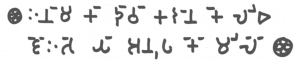
\includegraphics[scale=1.5]{content/fmatter/easteregg.pdf}

\noindent NAACL HLT 2015 Program Co-Chairs \\
Joyce Chai, Michigan State University \\
Anoop Sarkar, Simon Fraser University
